\documentclass[10pt, french]{beamer}
%\input{Beamer_ISEN.tex}
\usepackage[english, french]{babel}
\usepackage[utf8]{inputenc}
\usepackage[T1]{fontenc}
\usepackage{lmodern}
\usepackage{subfiles}
\usepackage{subfig}
\usepackage{amssymb}
\usepackage{amsmath}
\usepackage{eurosym}
\usepackage{amsfonts}
\usepackage{fontawesome}
\usepackage{amsthm}
\usepackage{upquote}
\usepackage{empheq}
\usepackage{bigints}
\usepackage{pdfpages}
\usepackage{fancyhdr}
\usepackage{textcomp}
\usepackage{etoolbox}
\usepackage{multirow}
\usepackage{xcolor}
\usepackage{alltt}
\usepackage{colortbl}
\usepackage{url}
\usepackage{placeins}
\usepackage{lastpage}
\usepackage{pgf-pie}
\usepackage{ulem}
\usepackage{mdframed}
\usepackage{hyperref}
\usepackage{xifthen}
\usepackage{ragged2e}
\usepackage{setspace}
\usepackage{iflang}
\usepackage{multimedia}
\usepackage{lcg}

\usetheme{Frankfurt}



%--- Header --------------------------------------------------------------------
\newcommand{\laclasse}{DEG}
\newcommand{\longtitle}{Statistique descriptive}
\newcommand{\shorttitle}{\textit{}}

\AtBeginSection[]
{
  \begin{frame}
  \frametitle{Sommaire}
  \tableofcontents[sectionstyle=show/shaded,subsectionstyle=hide]
  \end{frame} 
}
\AtBeginSubsection[]
{
  \begin{frame}
  \frametitle{Sommaire}
  \tableofcontents[sectionstyle=show/hide,subsectionstyle=show/shaded/hide]
  \end{frame} 
}
%--- Start document ------------------------------------------------------------
\begin{document}
\selectlanguage{french}
%\makeMyTitle
\title{Statistique descriptive}
\author{Vincent Tariel}
\institute{Université de la Nouvelle-Calédonie}
\date{09 Juillet 2020}
\begin{frame}
\titlepage
\end{frame}

\begin{frame}\frametitle{Avant-propos}
"Il y a trois sortes de mensonges : les mensonges, les sacrés mensonges et les statistiques."
Mark Twain\\
"Selon les statistiques, une personne sur quatre serait folle. Si vos trois meilleurs amis
ne le sont pas, alors c’est vous !" Rita Mae Brown \\
"Les lois de probabilités, si vraies en général,
si fallacieuses en particulier." Edward Gibbon \\
"La mort d’un homme est une tragédie. La
mort d’un million d’hommes est une
statistique." Joseph Staline\\
"Les statistiques nous montrent que parmi
ceux qui contractent l'habitude de manger,
très peu survivent." Wallace Irwin.
\end{frame}
\begin{frame}\frametitle{Devinette probabiliste}
\begin{itemize}
\item Ceci n’est pas un jeu de hasard, c’est un jeu sur le hasard.
\item Ci-dessous sont portées deux séries de cent chiffres. L’une
des deux séries est constituée à la main par quelqu’un à qui
il a été demandé d’écrire une suite de 0 et de 1. L’autre
correspond à une succession de tirages authentiques d’une
pièce de monnaie. (face=0, pile=1).
\item Série 1 :\\
01011011100111101010101011010100010101011111001\\
01010101110101000111100010100000111010101010001\\
101000.
\item Série 2 :\\
01101101110100110000111100000000000111010001010\\
11011000000101110001010000100001011111100011111\\
110010.
\end{itemize}
\end{frame}
\begin{frame}\frametitle{Devinette probabiliste}
\begin{itemize}
\item 
L'être humain est un piètre simulateur de hasard.
\item  On peut démontrer que la probabilité de présence
d'une suite de cinq 0 ou 1 dans une liste de cent
chiffres est supérieure à 97$\%$ or nous pensons, à
tort qu'une suite trop longue d'un même chiffre ne
fait pas très aléatoire. Cette remarque ne permet
pas ici d'identifier les séries.
\item  Avec six chiffres identiques, la probabilité est de
80$\%$. Seule la série 2 respecte ce critère.
\item   Seul le hasard peut permettre de donner une liste
de onze chiffres identiques$\dots$
\end{itemize}
Conclusion : ne pas se fier à son intuition en statistiques mais aux mathématiques ! 
\end{frame}



\begin{frame}\frametitle{Statistique descriptive}
Rôle :
\begin{itemize}
\item ressortir des propriétés de l'échantillon étudié,
\item suggérer des hypothèses
\end{itemize}
Méthodes d'analyse de données :
\begin{itemize}
\item représentation des données
\item classification pour réduire la taille de l'ensemble
d'individus (i.e. regrouper ceux qui se ressemblent
en « classes »)
\item factorielles pour réduire le nombre de variables
(i.e. analyse en composantes principales, analyse de
correspondances)
\end{itemize}
\end{frame}

%\begin{frame}\frametitle{Statistique inférentielle (ou décisionnelle)}
%Rôle :
%\begin{itemize}
%\item étendre les propriétés constatées sur un
%échantillon à toute la population
%\item Vérifier l'adéquation des hypothèses a priori ou
%issues d'une phase exploratoire
%\end{itemize}
%Méthodes :
%\begin{itemize}
%\item estimation d'une moyenne
%\item vérification d'une hypothèse (ou test)
%\item modélisation et prévision statistique
%\end{itemize}
%\end{frame}
\begin{frame}\frametitle{Historique}
Le mot “statistique” vient de l’allemand “Statistik”, qui, au milieu du
XVIIe siècle, désigne l’analyse des données utiles à l’´Etat. Le
traitement d’un grand nombre de données chiffrées qui sont triées,
classées ou résumées correspond à ce que l’on appelle aujourd’hui “les
statistiques” au pluriel. On les distingue de “la statistique”, au singulier,
qui correspond à la modélisation de ces données, vues comme résultats
d’expériences en présence d’aléa, et `a l’étude de cet aléa. On peut dater
l’émergence de la statistique du début du XIXe siècle, avec l’étude de
données provenant de l’astronomie sur les positions des planètes et leur
trajectoire. En particulier, en 1805 Adrien-Marie Legendre (1752-1832)
introduisit la méthode des moindres carrés pour estimer des coefficients
à partir de données, et en 1809 Carl Friedrich Gauss (1777-1855),
utilisant une modélisation des erreurs par la loi normale, retrouva en
maximisant la densité de la loi normale des erreurs.
\end{frame}
%\makeMyOutlines
%--- Section 1 -----------------------------------------------------------------

\section{Statistiques descriptives unidimensionnelle}
\subsection{Définitions de base}
\begin{frame}\frametitle{Définitions}
  Une étude statistique porte sur un ensemble d'objets ou de personnes appelé \alert{population}. \\
  
  En général, cet ensemble est trop grand pour que l'on interroge toutes les personnes. On se contente alors d'un certain nombre d'éléments de cet ensemble, appelés \alert{unités statistiques}. \\
  
  Pour chaque unité statistique, on pose une ou plusieurs questions qui correspondent à des \alert{caractères}. Un caractère peut être 
  \begin{itemize}
  \item qualitatif (la valeur est une catégorie) : couleur, profession, type de meuble, forme, etc.
  \item quantitatif (la valeur est un nombre) : nombre d'enfants, age, nombre de pièces, taille, poids, hauteur, largeur, salaire, etc.
  \end{itemize}
On note en général 
 \begin{itemize}
 \item $i$ un indice qui représente le numéro de l'unité statistique
 \item $x_i$ la valeur du premier caractère mesuré sur l'unité statistique $i$
 \item $y_i$ la valeur du deuxième caractère mesuré sur l'unité statistique $i$
 \end{itemize}  
\end{frame}
\begin{frame}\frametitle{Exemples}
  \textbf{Sujet : notes de l'évaluation de l'enseignement statistique}
  \begin{itemize}
  \item Population : licence DEG
  \item Unité statistique : étudiant
  \item Caractère : note de 0 à 20(quantitatif)
  \end{itemize}
$x_i$ est la note de l'étudiant d'indice $i$. 
%  \begin{figure}
%    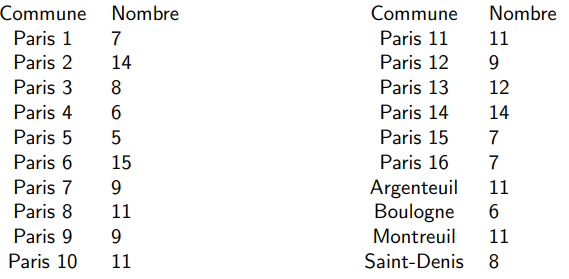
\includegraphics[width=0.45\textwidth]{Images/entreprise.png}
%  \end{figure}
\end{frame}
\subsection{Représentations des données}
\begin{frame}
  \frametitle{Tableaux de données}
  \begin{itemize}
\item  \textbf{Liste}\\ 0 10 17 2 15 19  6 17 15 0 19 10 12 19 0 10 4 6 12 9 17 \\
\item  \textbf{Effectif}\\
\begin{tabular}{ccccccccccc}
Valeurs  & 0 &2 & 4&6&9&10&12&15&17&19\\
Effectifs &3  & 1& 1&2&1&3&1&2&3&3
\end{tabular}
\item  \textbf{Fréquence}\\
\hspace{-2cm}\begin{tabular}{rcccccccccc}
Valeurs  & 0 &2 & 4&6&9&10&12&15&17&19\\
Fréquence &0,15  & 0,05& 0,05 &0,1&0,05&0,15&0,05&0,1&0,15&0,15
\end{tabular}
\item  \textbf{classes et fréquences}\\
\begin{tabular}{rcccc}
Valeurs  & [0,5[ &[5,10[&[10,15[&[15,20[\\
Fréquence & 0,25&0,15&0,20&0,4
\end{tabular}
  \end{itemize}
\end{frame}
\begin{frame}
  \frametitle{Histogramme}
  \begin{figure}
    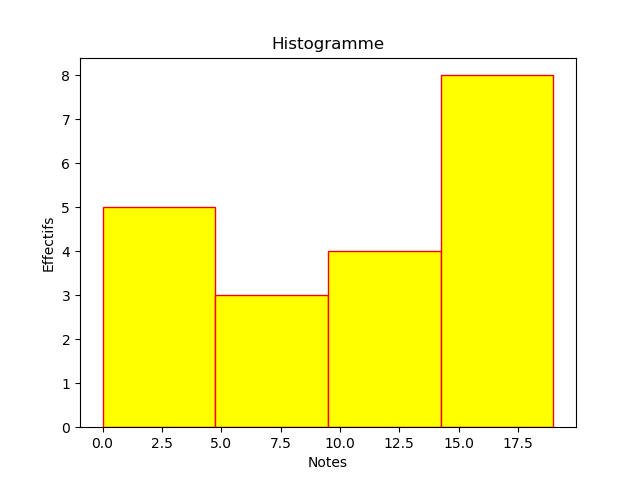
\includegraphics[width=0.9\textwidth]{Images/note.png}
  \end{figure}
Un quart de la classe est en grande difficulté avec des notes <5 et de nombreux élèves 2/5 ont très bien réussi l'évaluation avec note $\geq 15$.  
\end{frame}
%\begin{frame}\frametitle{Représentations de données : diagramme en bâtons}
%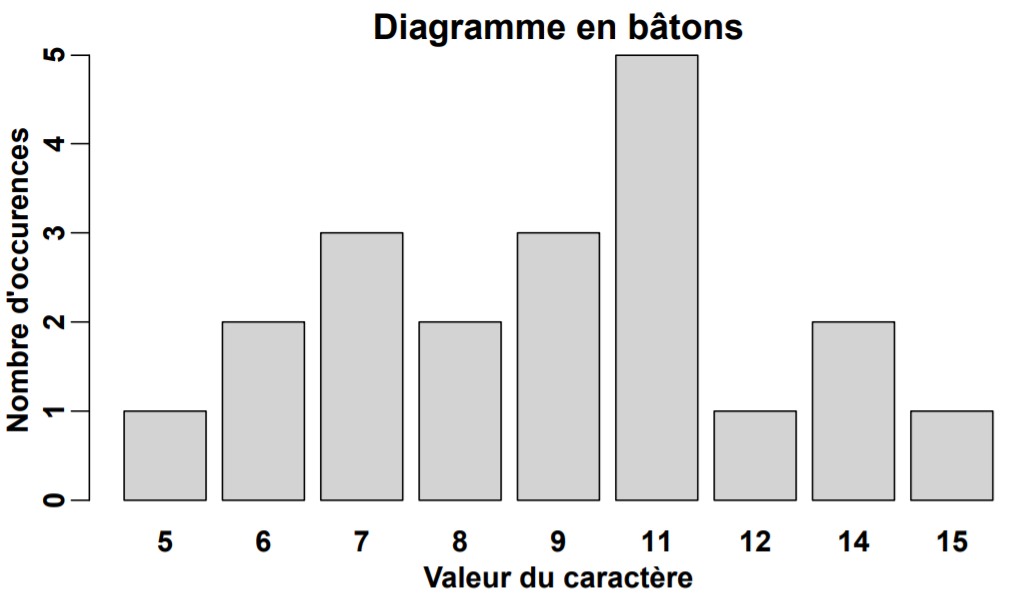
\includegraphics[width=4.5in]{Images/DiagrammeBaton.png}
%\end{frame}
%
%\begin{frame}\frametitle{Représentations de données : diagramme en bâtons}
%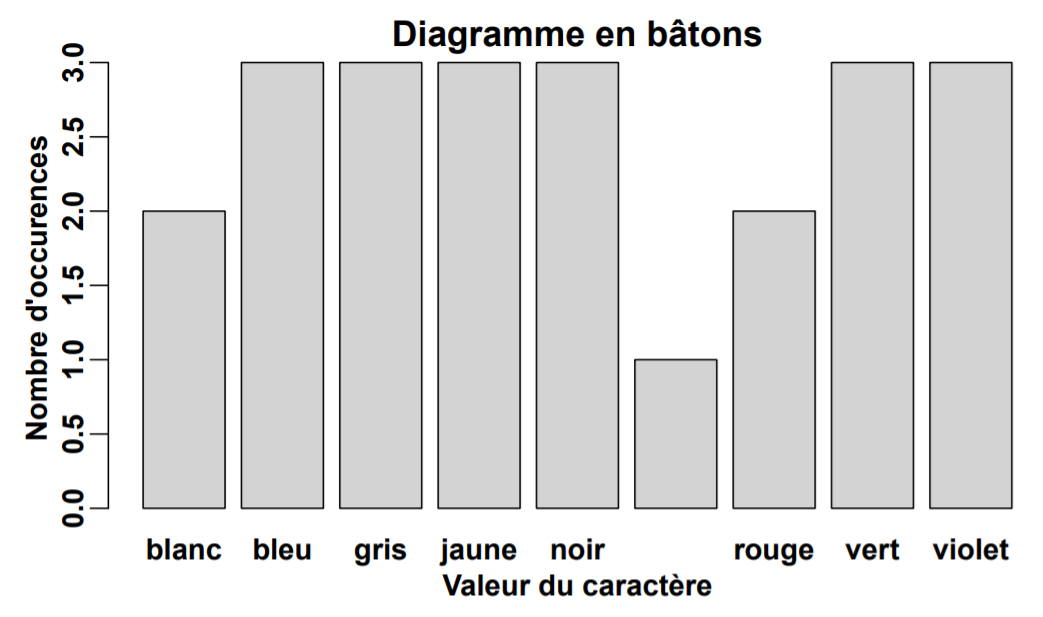
\includegraphics[width=4.5in]{Images/DiagrammeBaton1.png}
%\end{frame}

%\begin{frame}\frametitle{Représentations de données : histogramme}
%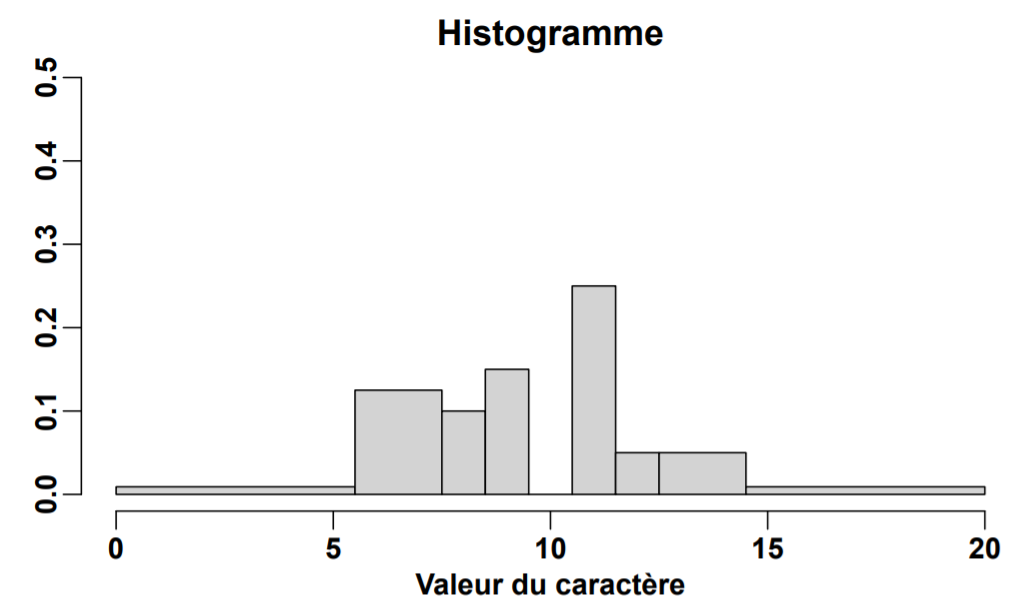
\includegraphics[width=4.5in]{Images/histogramme.png}
%\end{frame}
%\begin{frame}\frametitle{Représentations de données : histogramme}
%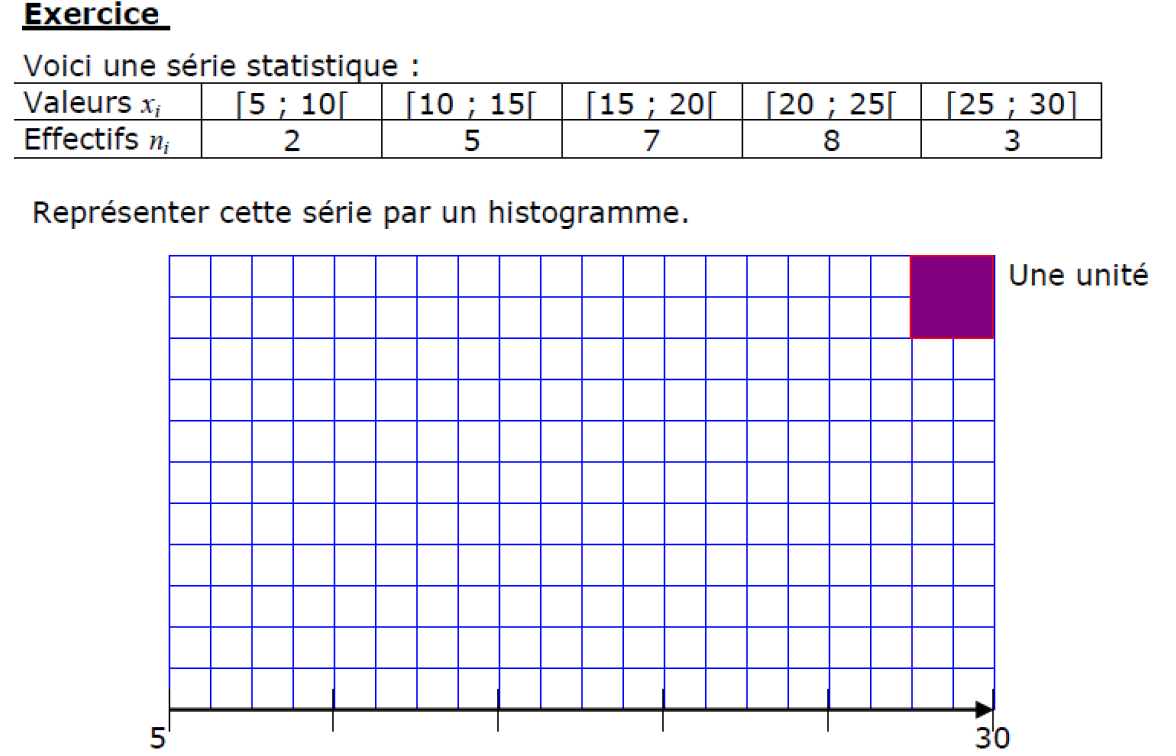
\includegraphics[width=4.5in]{Images/histogramme_exo.png}
%\end{frame}
%\begin{frame}\frametitle{Représentations de données : histogramme}
%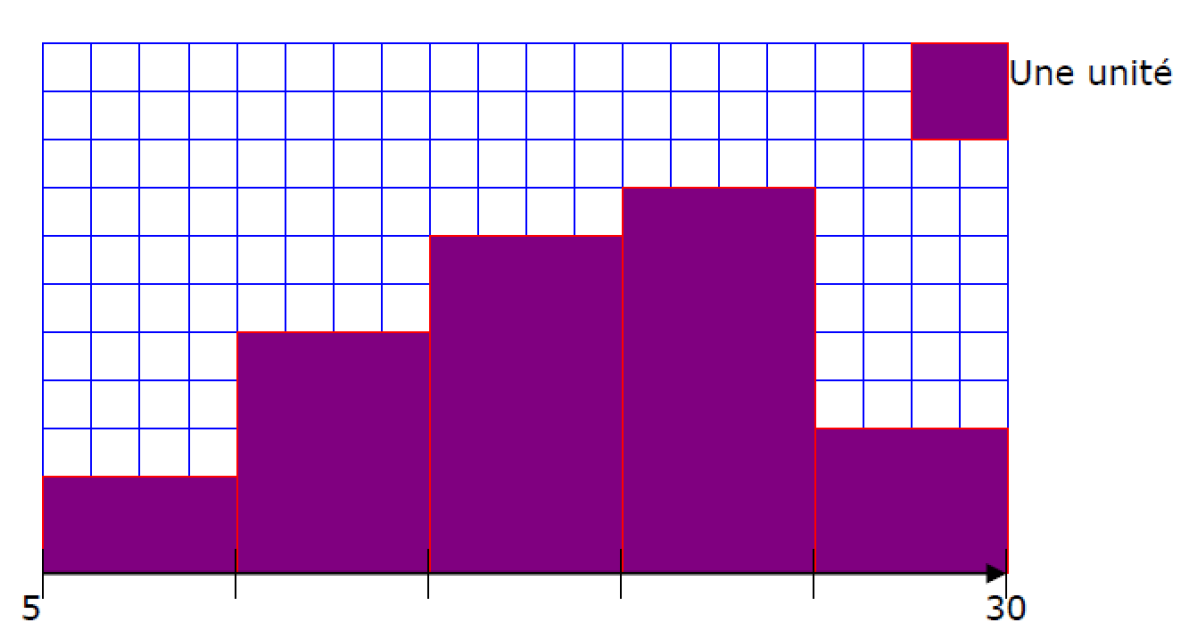
\includegraphics[width=4.5in]{Images/histogramme_exo_cor.png}
%\end{frame}
\begin{frame}\frametitle{Histogramme}
\textbf{Nombre de classes :}\\
Le nombre de classes dépend du nombre de valeurs N dont on dispose.\\
Le nombre de classes K peut être déterminé par les formules suivantes :
$$K=\sqrt{N} \text{ ou } K=1+\log _{2}N.$$\\
\textbf{Taille de l'intervalle :}\\
Généralement, dans le cadre d'une analyse de ce type,
on utilise des classes de largeur identique.\\
\end{frame}
\begin{frame}\frametitle{Représentations de données : histogramme}Soit la fabrication de rations alimentaires, la pesée des rations avant emballage donne la série de mesures suivantes en kg :\\
\begin{tiny}
0,547	0,563	0,532	0,521	0,514	0,547	0,578	0,532	0,552	0,526	0,534	0,560	0,502	0,503	0,516	0,565
0,532	0,574	0,521	0,523	0,542	0,539	0,543	0,548	0,565	0,569	0,574	0,596	0,547	0,578	0,532	0,552
0,554	0,596	0,529	0,555	0,559	0,503	0,499	0,526	0,551	0,589	0,588	0,568	0,564	0,568	0,556	0,523
0,526	0,579	0,551	0,584	0,551	0,512	0,536	0,567	0,512	0,553	0,534	0,559	0,498	0,567	0,589	0,579
\end{tiny}\\
Les caractéristiques du relevé sont les suivantes :
\begin{enumerate}
\item Le nombre d'échantillons : N=64
\item L'étendue : w=0,098 kg
\item Valeur minimale : 0,498 kg
\item Valeur maximale : 0,596 kg
\end{enumerate}
On en déduit les paramètres suivants pour l'histogramme :
\begin{enumerate}
\item  Le nombre de classes est de 7 (en utilisant la formule avec le logarithme)
\item L'amplitude de classe est 0,098/7 = 0,014 kg que l'on arrondit à 0,015 kg (résolution de la balance : 0,001 kg)
\item La valeur minimale de la première classe est de 0,498 – (0,001/2) = 0,4975. Par souci de facilité pour l'interprétation, on peut arrondir cette valeur à 0,495 kg.
\end{enumerate}
\end{frame}
\begin{frame}\frametitle{Histogramme}
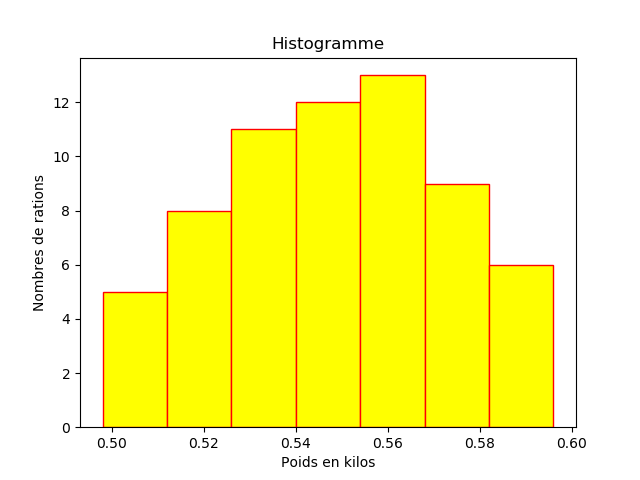
\includegraphics[width=3.in]{Images/histogramme_exo2_cor.png}
\end{frame}

\subsection[Moyenne et variance]{Moyenne, variance et écart-type}
\begin{frame}{Moyenne}
\begin{block}{Moyenne}
La moyenne d'une série statistique noté $\bar x$ est le quotient  de la somme de toutes les valeurs de cette série par l'effectif total :
$$\bar x =\frac 1 N \sum_{i=1}^N x_i$$
La moyenne exprime la valeur qu’aurait chacun si le partage était équitable.
\end{block}
Exemple des notes :
$$\bar x =\frac{0+  10 +\dots + 17}{20}=10,35$$
Avec le tableau des effectifs, le calcul est :
$$\bar x =\frac{3\times 0+  1 \times 2+\dots +  3\time 19}{20}=10,35$$
\end{frame}

\begin{frame}{Variance et écart-type}
\begin{block}{Moyenne}
L'écart d'une série statistique noté $\sigma$ est  la racine carrée de la variance, $V$, c'est-à-dire :
$$ \sigma ={\sqrt {V}}={\sqrt {{\frac {1}{N}}\sum _{i=1}^{N}(x_{i}-{\overline {x}})^{2}}}$$
La moyenne est une mesure de la dispersion des valeurs d'un échantillon statistique. 
\end{block}
Exemple des notes :
$$\sigma =\frac{ (0-10,35)^2+  (10-10,35)^2 +\dots + (17-10,35)^2}{20}=6,61$$
Avec le tableau des effectifs, le calcul est :
$$\sigma =\frac{3\times (0-10,35)^2+  1 \times (2-10,35)^2+\dots +  3\times (19-10,35)^2}{20}=6,61$$
Comme l'écart type est de $6,61$, les notes sont très étalées. 
\end{frame}
\subsection[Répartition et quantile ]{Quantiles et boîte à moustache}
\begin{frame}{Quantile}
\begin{block}{Quantile}
Les quantiles sont les valeurs qui divisent un jeu de données en intervalles contenant le même nombre de données. Ainsi les quartiles sont les trois quantiles qui divisent un ensemble de données en quatre groupes de taille égale. La médiane quant à elle est le quantile qui sépare le jeu de données en deux groupes de taille égale.
\end{block}
%  \textbf{Définition} $F(t)$ est le nombre de valeurs inférieures ou égales à $t$ exprimé en fréquence.
%  \[ F(t) = \mathbb{P}(X \leq t).\]
%\textbf{Fréquence}\\
%\hspace{-2cm}
Pour déterminer les quartile $q_1$ et $q_3$ et la médiane, on calcul le tableau des fréquences cumulées :
\hspace*{-2cm}\begin{tabular}{rcccccccccc}
Valeurs  & 0 &2 & 4&6&9&10&12&15&17&19\\
Fréquences &0,15  & 0,05& 0,05 &0,1&0,05&0,15&0,05&0,1&0,15&0,15\\
Fréquences cumulées&0,15  & 0,2& 0,25 &0,35&0,4&0,55&0,6&0,7&0,85&0,1
\end{tabular}
Pour le premier quartile on cherche la valeur telle que la fréquence cumulée dépasse 0,25 pour la première fois, soit $q_1=4$. \\
Pour le troisième quartile, 0,75 pour la première fois, soit $q_3=17$. \\
Pour la médiane, 0,5 pour la première fois, soit $M=10$. \\

\end{frame}
%\begin{frame}{Quantiles}
%  \textbf{Définition} On appelle \alert{quantile d'ordre $\alpha$}  la plus petite valeur du caractère telle que $\mathbb{P}(X \leq q_\alpha) \geq \alpha$. La fonction quantile est la réciproque de la fonction de répartition.\\
%  Valeurs particulières : 
%  \begin{itemize}
%  \item la \alert{médiane} est $q_{0.5}$.
%  \item le 1er quartile est $q_{0.25}$, le 2e quartile est la médiane, le 3e quartile est $q_{0.75}$
%  \item le 1er décile est $q_{0.1}$, le 3e décile est $q_{0.3}$, etc.
%  \end{itemize}
%    \textbf{Exemple : (données en liste)}\\
%    Données : 7 14 8 6 5 15 9 11 9 11 11 9 12 14 7 7 11 6 11 8 \\
%    Fonction de répartition : \\
%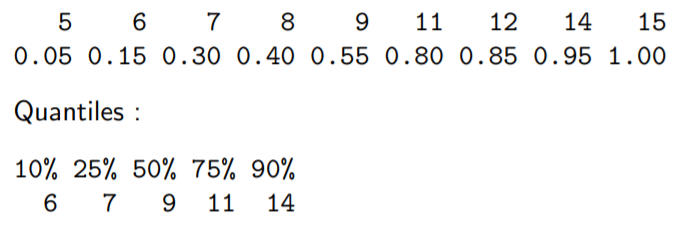
\includegraphics[width=2.5in]{Images/quantile.png}
%\end{frame}
\begin{frame}{Boîte à moustache}
\begin{block}{Boîte à moustache}
la boîte à moustaches est un moyen rapide de figurer le profil essentiel d'une série statistique quantitative en représentant  quelques indicateurs de position du caractère étudié (médiane, quartiles, minimum, maximum ou déciles). Ce diagramme est utilisé principalement pour comparer un même caractère dans deux populations de tailles différentes.
\end{block}
Il s'agit de tracer un rectangle allant du premier quartile au troisième quartile et coupé par la médiane. Ce rectangle suffit pour le diagramme en boîte. On peut rajouter des segments aux extrémités menant jusqu'aux valeurs extrêmes, ou jusqu'aux premier et neuvième déciles $({\displaystyle D_{1}/D_{9}})$.
\end{frame}

\begin{frame}{Boite à moustache}
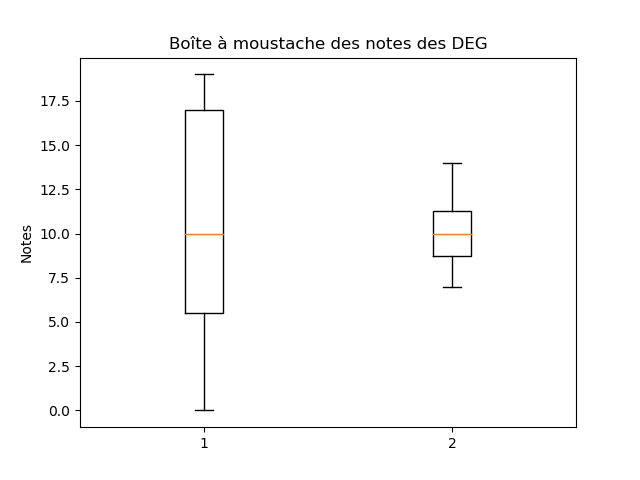
\includegraphics[width=3.5in]{Images/boite.png}\\
Les notes  de la première évaluation sont nettement plus hétérogènes que les notes de la seconde évaluation.  
\end{frame}
%\subsection[Coefficient d'asymétrie]{Coefficient d'asymétrie}
%\begin{frame}{Coefficient d'asymétrie}
%Étant donnée une variable aléatoire réelle $X$ de moyenne $\mu$ et d'écart type $\sigma$, on définit son coefficient d'asymétrie comme le moment d'ordre trois de la variable centrée réduite :
%$$ \gamma _{1}=\mathbb {E} \left[\left({\frac {X-\mu }{\sigma }}\right)^{3}\right]$$
%\begin{itemize}
%\item Un coefficient nul indique une distribution symétrique.
%\item Un coefficient négatif indique une distribution décalée à droite de la médiane, et donc une queue de distribution étalée vers la gauche.
%\item Un coefficient positif indique une distribution décalée à gauche de la médiane, et donc une queue de distribution étalée vers la droite.
%\end{itemize}
%\end{frame}
%\begin{frame}{Coefficient d'asymétrie}
%Une enquête menée auprès de 1500 ménages d'une certaine région géographique rurale s'est intéressée à la variable $X$ correspondant à la taille du ménage, c'est-à-dire au nombre de personnes constituant le ménage. Les données recueillies peuvent être présentées sous la forme du diagramme en bâtons suivant.\\
%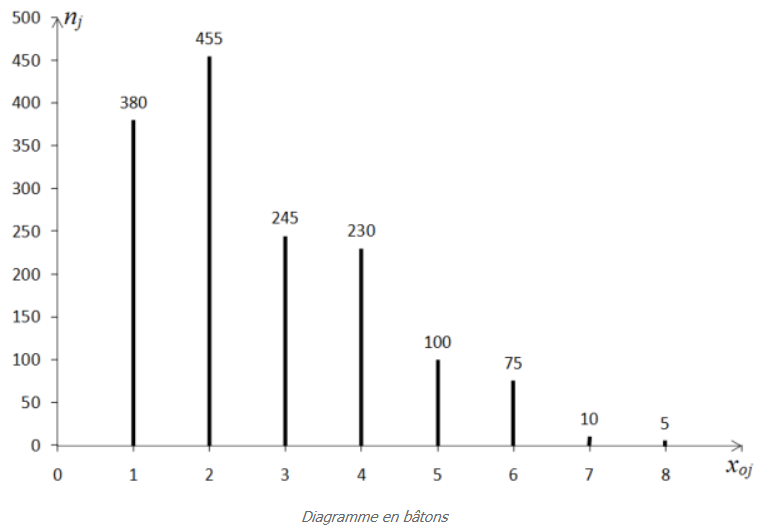
\includegraphics[width=2.5in]{Images/asym_exo.png}
%\end{frame}
%\begin{frame}{Coefficient d'asymétrie}
%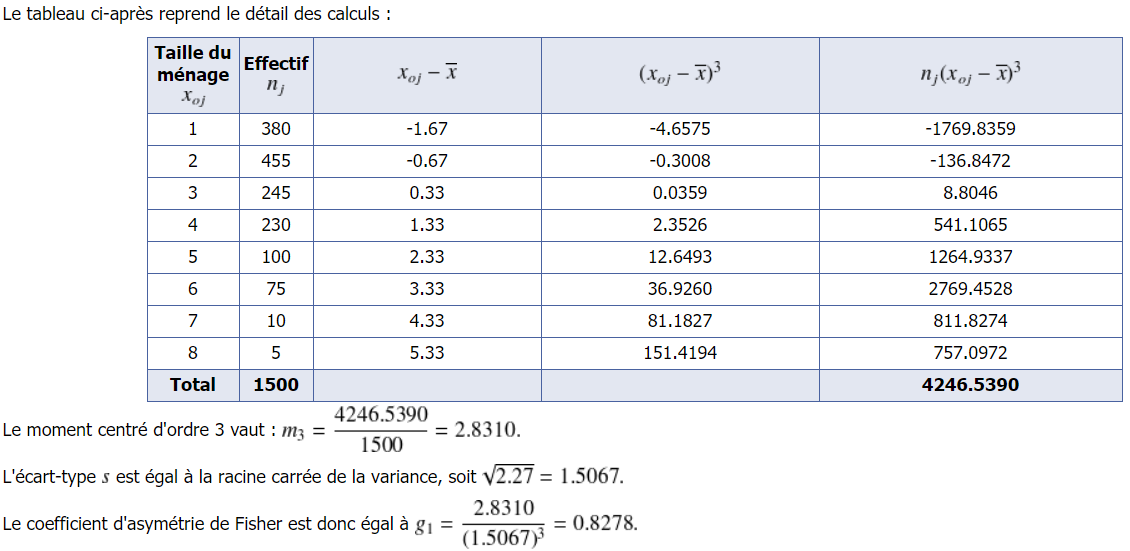
\includegraphics[width=4.5in]{Images/asym_exo_cor.png}
%\end{frame}

\section{Statistiques descriptives bidimensionnelle}
\subsection{Représentations des données}
\begin{frame}{Nuage de points}
\begin{block}{Nuage de points}
Le nuage de points, aussi appelé diagramme de dispersion, est la représentation graphique d'une série statistique à deux variables. Il permet d'observer la relation entre ces deux variables. Il est possible d'effectuer un ajustement de ce nuage de points par une courbe afin d'effectuer des prévisions.
\end{block}
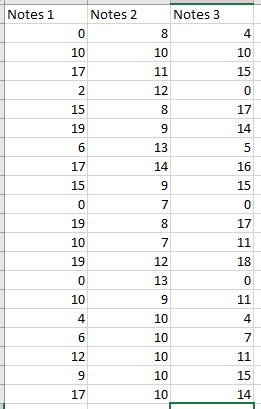
\includegraphics[width=1.2in]{Images/data.png}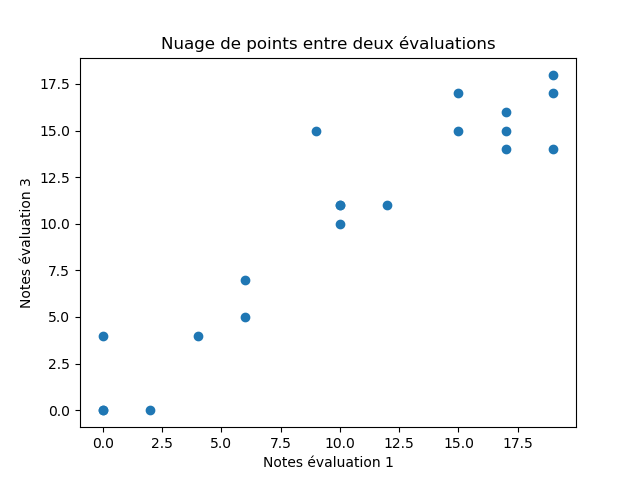
\includegraphics[width=2.7in]{Images/nuage_note.png}
\end{frame}
\subsection{Lien statistiques entre deux variables}
\begin{frame}{Corrélation et causalité}
\begin{itemize}
\item Coluche : " 1/3 des accidents de la route étant dus à des conducteurs alcooliques, 
qu'est ce qu'on attend pour punir les 2/3 de conducteurs sobres responsables de la majorité des accidents ? "
\item "Une étude anglaise a prouvé que les gens habitant près de pylônes à haute tension étaient significativement plus souvent malades que le reste de la population. Est-ce la faute du courant électrique ? Ce n'est pas évident parce qu'une autre étude a révélé que les habitants sous les pylônes étaient en moyenne plus pauvres ; et on sait les liens santé-pauvreté... À elle seule, cette étude ne permet pas de conclure."
\end{itemize}
L'objectif est de déterminer un \textit{corrélation} entre deux variables $X$ et $Y$, étudiées sur le même échantillon. Dans certains
cas, cette liaison peut être considérée a priori comme causale, une variable $X$
expliquant l'autre $Y$ ; dans d'autres, ce n'est pas le cas, et les deux variables
jouent des rôles symétriques. Dans la pratique, il conviendra de bien différencier les deux situations et une liaison n'entraîne pas nécessairement une
causalité.
\end{frame}

\begin{frame}{Corrélation}
\begin{block}{Corrélation}
La corrélation entre deux variables aléatoires $(X,Y)$ est une notion de liaison qui contredit leur indépendance.\\
A $X=x$ fixé, la moyenne $\bar Y$ est une fonction de $x$.\\
Cette corrélation est très souvent réduite à la corrélation linéaire entre variables quantitatives, c'est-à-dire l'ajustement d'une variable par rapport à l'autre par une relation affine obtenue par régression linéaire.
\end{block}
\end{frame}
\begin{frame}{Corrélation}
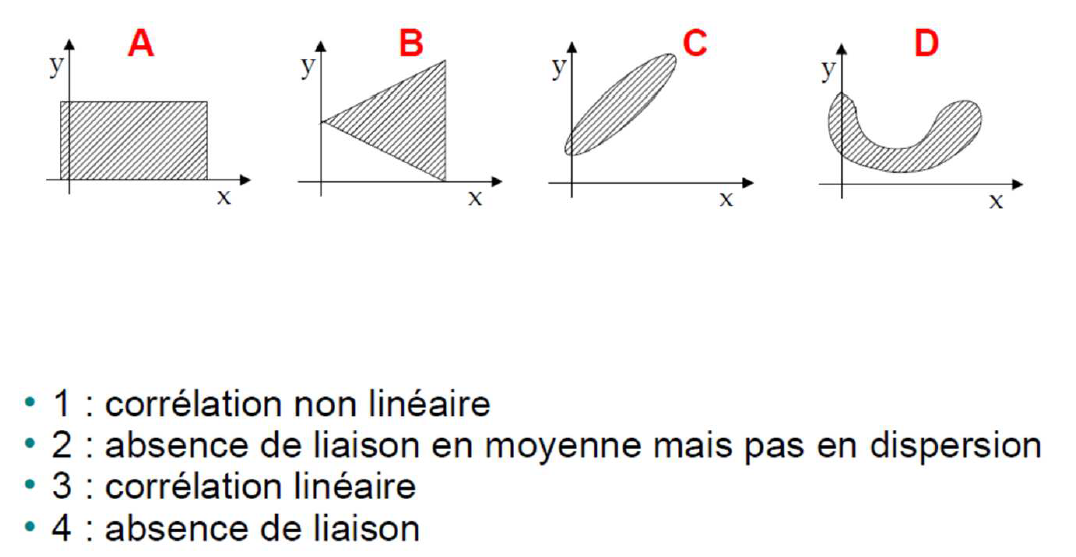
\includegraphics[width=4.5in]{Images/corr.png}
\end{frame}
\begin{frame}{Coefficient de corrélation}
Partant d'un échantillon $ \{(x_{i},y_{i})\,|\,1\leq i\leq N\}$ de réalisations indépendantes de deux variables $X$ et $Y$, le coefficient de corrélation est donné par

$$r=\dfrac {Cov(X,Y)}{{\sigma }_{X}{\sigma }_{Y}}$$
avec
$$Cov(X,Y)={\frac {1}{N}}\sum _{i=1}^{N}(x_{i}-{\bar {x}})\cdot (y_{i}-{\bar {y}})$$
$$\sigma_{X}=\sqrt {{\dfrac {1}{N}}\displaystyle \sum _{i=1}^{N}(x_{i}-{\bar {x}})^{2}}$$
$$\sigma_{Y}=\sqrt {{\dfrac {1}{N}}\displaystyle \sum _{i=1}^{N}(y_{i}-{\bar {y}})^{2}}$$
\end{frame}
\begin{frame}{Coefficient de corrélation}
\hspace{-0.8cm}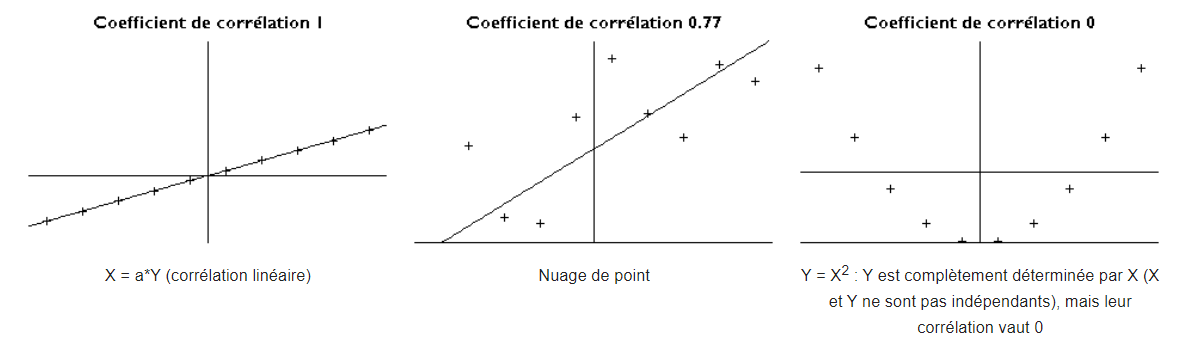
\includegraphics[width=4.5in]{Images/corr_fig.png}
\end{frame}
\begin{frame}{Régression linéaire}
Dans le cadre d'un modèle linéaire simple, on peut représenter graphiquement la relation entre x et y à travers un nuage de points. L'estimation du modèle linéaire permet de tracer la droite de régression, d'équation $y=\beta _{0}+\beta _{1}x$. Le paramètre $\beta _{0}$ représente l'ordonnée à l'origine et $\beta _{1}$ le coefficient directeur de la droite.
On  exprime $\beta _{0}$ et $\beta _{1}$ ainsi :
$$\beta_{1}={\frac {\operatorname {cov} (\mathrm {X} ,\mathrm {Y} )}{\operatorname {var} (\mathrm {X} )}}$$
$$\beta_0 =E(Y) - \beta_1 E(X)$$
Partant d'un échantillon $ \{(x_{i},y_{i})\,|\,1\leq i\leq n\}$, on a :
$$\beta_{1}={\frac {\sum (x_{i}-{\bar {x}})(y_{i}-{\bar {y}})}{\sum (x_{i}-{\bar {x}})^{2}}}$$
$$\beta_{0}={\frac {\sum y_{i}-{\hat {\beta }}_{1}\sum x_{i}}{n}}$$
\end{frame}
\begin{frame}{Régression linéaire}
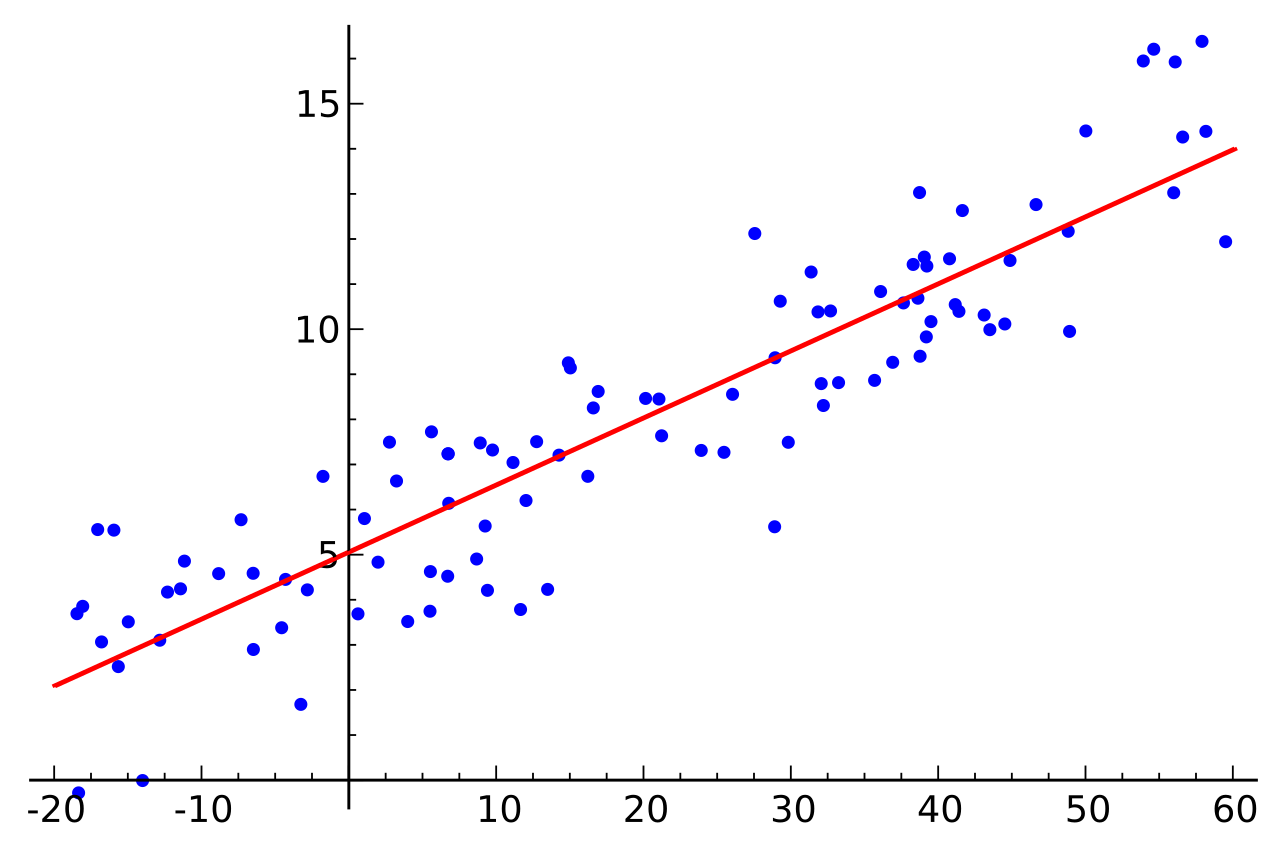
\includegraphics[width=4in]{Images/linear_regression.png}
\end{frame}
\begin{frame}{Régression linéaire}
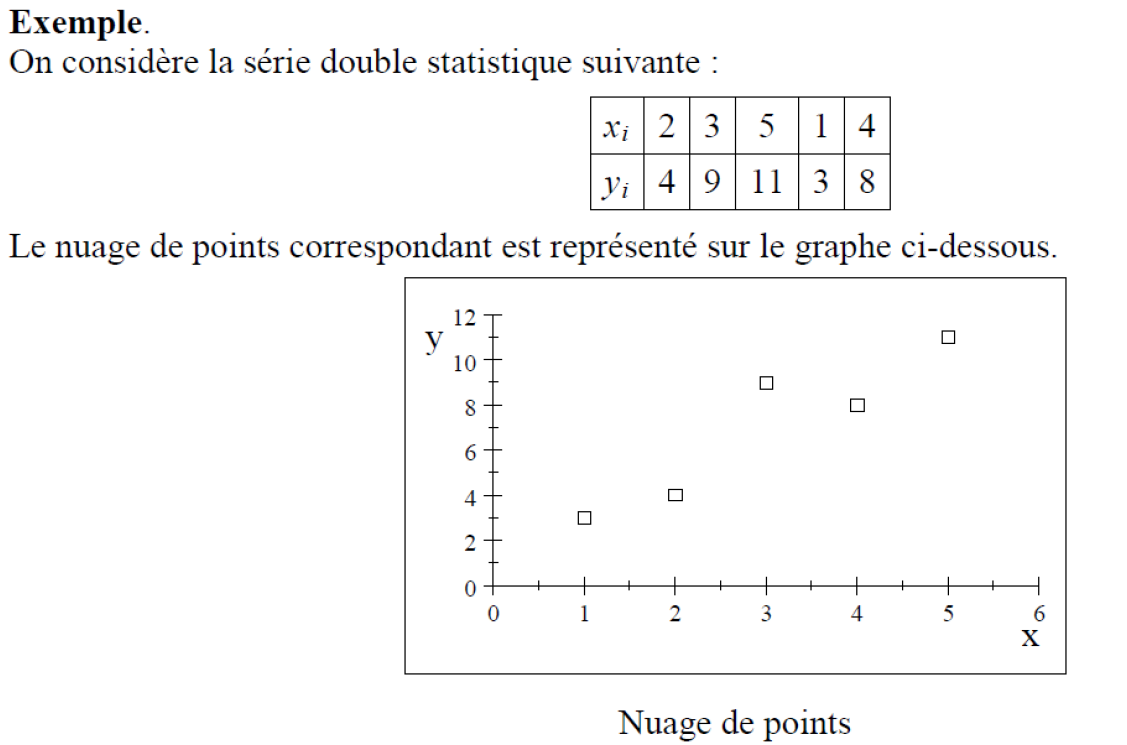
\includegraphics[width=4in]{Images/reg_exo.png}
\end{frame}
\begin{frame}{Régression linéaire}
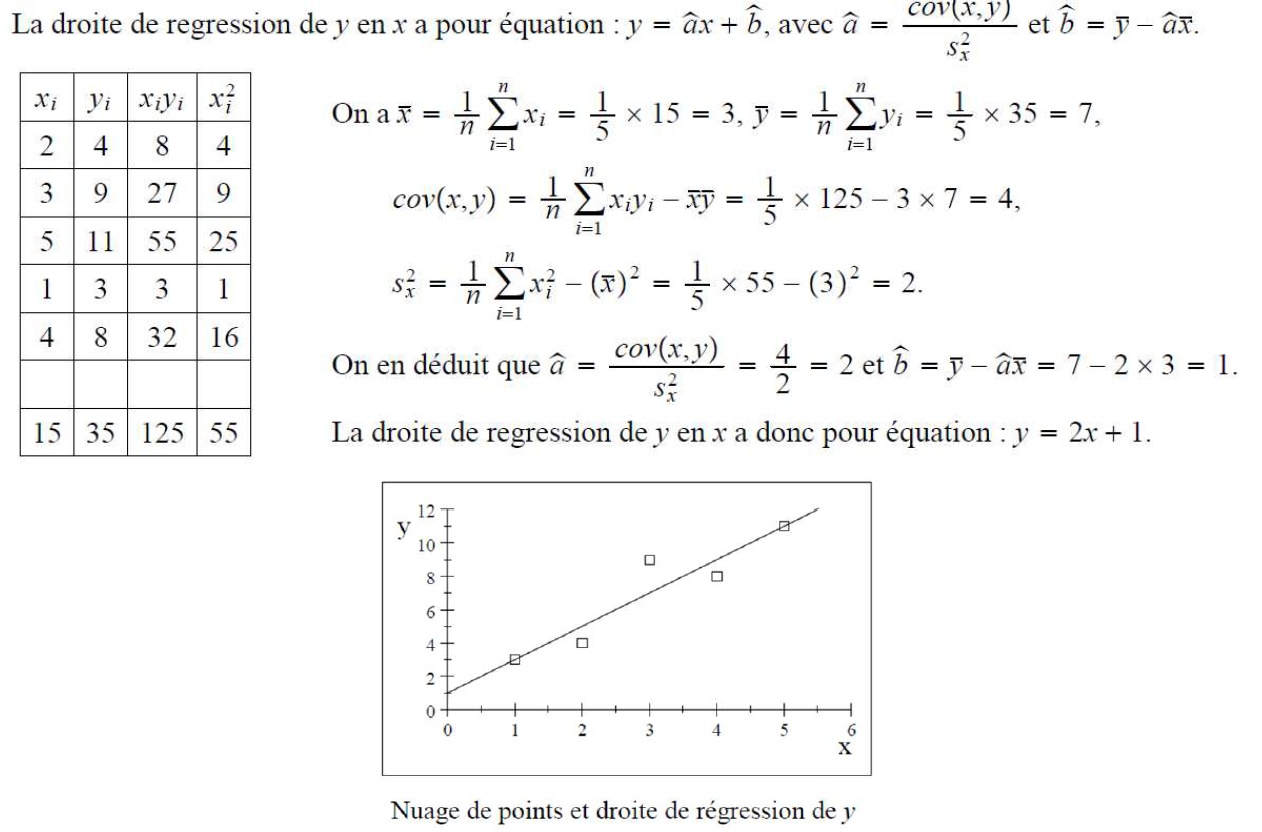
\includegraphics[width=4in]{Images/reg_exo_cor.png}
\end{frame}
\begin{frame}{Régression linéaire}
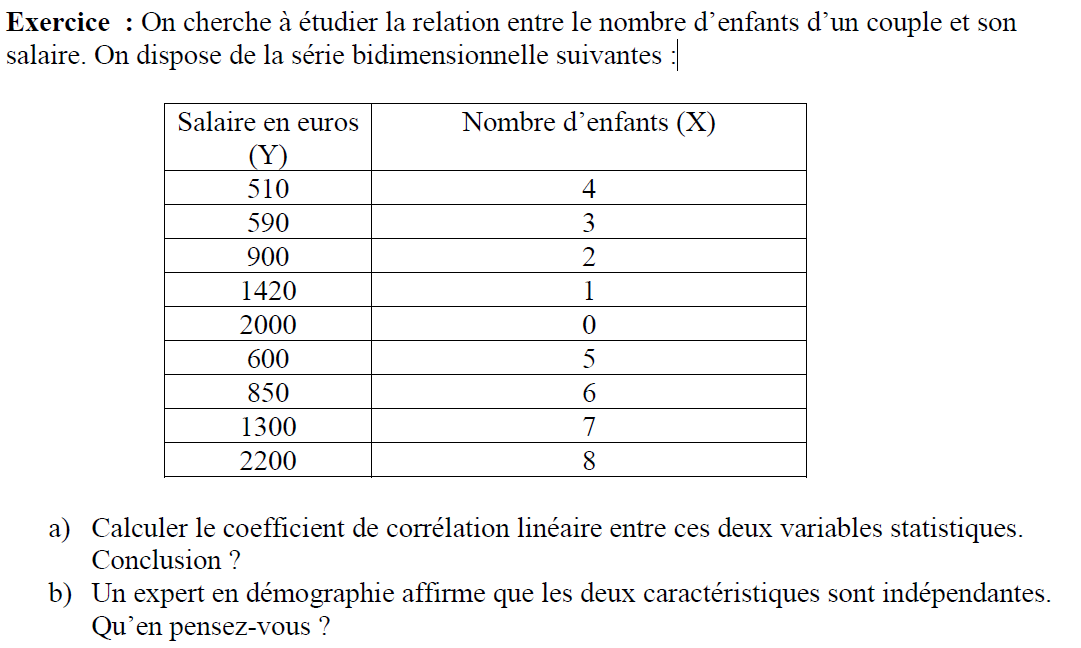
\includegraphics[width=4in]{Images/reg_exo1.png}
\end{frame}
%\makeMyQuestions

\end{document}
